\section{Methods}
\label{sec:methods}

This section details the friction identification procedure which starts with data acquisition from joint movements, followed by data processing to ensure the quality and relevance of the data. We adopt both static known models, such as CV and SCV, as well as a data-driven model, the PINN model. The aim is to accurately predict friction to improve joint torque control performance.
\looseness=-1

\begin{figure}[t]
    \centering
    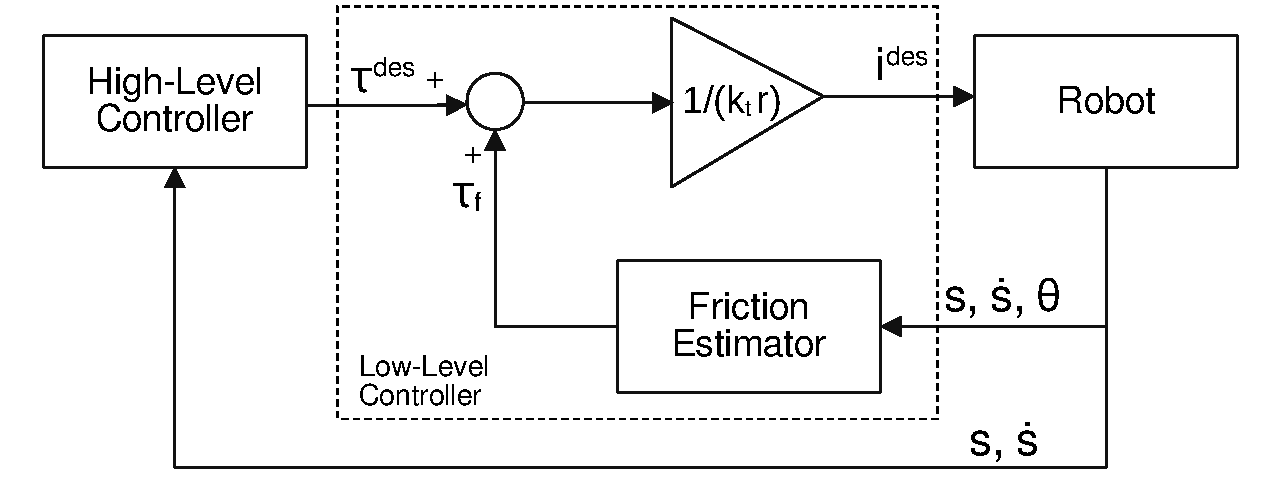
\includegraphics[width=1.0\linewidth]{figures/controlschema.pdf}
    \caption{Block diagram of the two-layer controller architecture. The PINN implements the block Friction Estimator of the Low-Level controller.}
    \label{fig:controlarchitecture}
    \vspace{-20pt}
\end{figure}

\subsection{Data acquisition procedure}
The selection of the input excitation signal is a critical factor that determines the quality and accuracy of the estimated friction model, as well as the richness of the acquired data. A well-designed excitation signal captures the fundamental features of the system dynamics.
Experiments are conducted by generating desired motor current trajectories using a simple parameterized controller, with data acquired simultaneously on multiple joints. The sine waves exhibit increasing amplitudes and frequencies. Specifically, for each fixed amplitude value, we vary the frequency from its minimum to its maximum value. The minimum and maximum amplitudes and frequencies depend on the specific joint. Ramp signals are used with varying increments for each experiment. The trajectory is stopped when the motor current reaches the joint-dependent maximum value or when the joint position approaches its hardware limit. The final trajectory is represented by steps. Specifically in each experiment, we apply a step change in the motor current and each step is maintained for a few seconds. The trajectory is halted either after the specified duration or when the joint position approaches its hardware limit. To ensure that all potential static friction variations, which may arise from different initial configurations of the harmonic drive, are accounted for, each experiment is repeated multiple times starting from different initial joint configurations.
\looseness=-1

The generated motor currents are subsequently applied to a low-level PI motor current controller running at 20 KHz.
Data are logged at 500 Hz and then offline resampled at 1000 Hz for friction identification purposes. This resampling is necessary because the friction estimator is then integrated with a low-level joint torque controller running online at 1000 Hz on the robot computer.
\looseness=-1

\subsection{Data preprocessing}
Data pre-processing is essential to reduce measurement noise and outliers and generate joint velocities and accelerations. A low-pass Butterworth filter is employed to reduce the noise of measured motor currents and Inertia Measurement Units (IMU) signals~\cite{mahata2018optimal}. Joint velocities and accelerations are derived from collected joint positions using a Kalman Filter~\cite{welch1995introduction}. The tuning of these filters is straightforward, aiming to remove noise without losing important information.
Another critical data processing objective is to compute joint torques, which are not directly measured due to the absence of joint torque sensors on our humanoid robot. Joint torques can be computed based on the knowledge of the robot state and the robot model from Eq.~\ref{eq:robotdynamics}~\cite{traversaro2017thesis}. The friction torques, representing the ground truth ($\tau_{F, \text{true}}$) for the estimation algorithm, are computed from Eq.~\eqref{eq:HDmodel} as $\tau_{F, \text{true}} = r k_t i_m - \tau $ where the joint torque $ \tau $ is given by Eq.~\eqref{eq:robotdynamics}.
\looseness=-1


\subsection{PINN architecture}

\looseness=-1
The friction model is estimated using a Physics-Informed Neural Network (PINN). The joint velocity ($\dot{s}$) and the position error ($\Delta \theta = r s - \theta$) are buffered in a joint state history within a finite time window. The use of the position error ensures the model can differentiate between situations where the joint is stationary due to friction and cases where no movement is commanded, reflecting whether the motor intends to move or remain still. The PINN maps the joint state to a frictional torque value ($\tau_F$).
The loss function used to train the PINN combines both data-driven and physics-based components~\eqref{eq:loss} and is defined as
\begin{equation}
\begin{aligned}
&\mathcal{L}_{\text{data}} =  (1 - \lambda) \frac{1}{N} \sum_{i=1}^{N} \left( \tau_{F, \text{pred}} - \tau_{F, \text{true}} \right)^2 \\
&\mathcal{L}_{\text{physics}} = \lambda \frac{1}{M} \sum_{j=1}^{M} \left( \tau_{F, \text{pred}} - \tau_{F, \text{physics}} \right)^2 \; ,
\end{aligned}
\label{eq:combined_loss}
\end{equation}
where $\lambda \in [0, 1]$ is the regularization parameter, $\tau_{F, \text{physics}}$ is defined by~\eqref{eq:scv}, and $\tau_{F, \text{true}}$ is computed from \eqref{eq:HDmodel}.
\looseness=-1

This loss function ensures that the PINN predictions are accurate for the data and consistent with the underlying physics of the SCV model. The PINN consists of 2 hidden layers with \textit{ReLU} activation, incorporating dropout after each layer, and a linear output layer. We utilize the Weight and Biases (W\&B) platform to optimize the hyperparameters of our PINN model~\cite{wandb}. W\&B seamlessly integrates with TensorFlow and PyTorch, employing advanced techniques for hyperparameter optimization. We use the Random Search algorithm to select the set of hyperparameters from a specified search space~\cite{bergstra2012random}. Our objective is to identify the parameters yielding optimal performance by minimizing validation loss. Key parameters optimized include batch size, hidden layer sizes, learning rate, history length, regularization parameter $\lambda$, and dropout rate, with the number of epochs fixed.
\looseness=-1

\subsection{Controller architecture}
The control architecture is shown in Fig. \ref{fig:controlarchitecture} and is detailed below.
\looseness=-1

\subsubsection{High-Level Control}
\label{sec:HLC}
Based on the robot dynamics~\eqref{eq:robotdynamics}, the high-level control law computes the desired joint torques $\tau_{des}$ solving a constrained quadratic programming problem (QP). The implemented QP is a simplified version of the problem defined in~\cite{romualdi2022whole} and considers only the joint position regularization task in the control problem.
This task prevents huge variations of the desired joint accelerations and is described by \mbox{$\Psi_{s} = \ddot{s}^{*} - \begin{bmatrix} 0_{n \times 6}  & I_{n}  \end{bmatrix} \dot{\nu}$}. $\ddot{s}^{*}$ is defined as \scalebox{0.8}{$\ddot{s}^{*} = \ddot{s}^{des} + K_d (\dot{s}^{des} - \dot{s}) + K_p (s^{des} -s)$}, where $s^{des}$ is the desired joint trajectory, and $K_d$ and $K_p$ are two positive-defined diagonal matrices.
\looseness=-1

\begin{figure}[t]
    \centering
    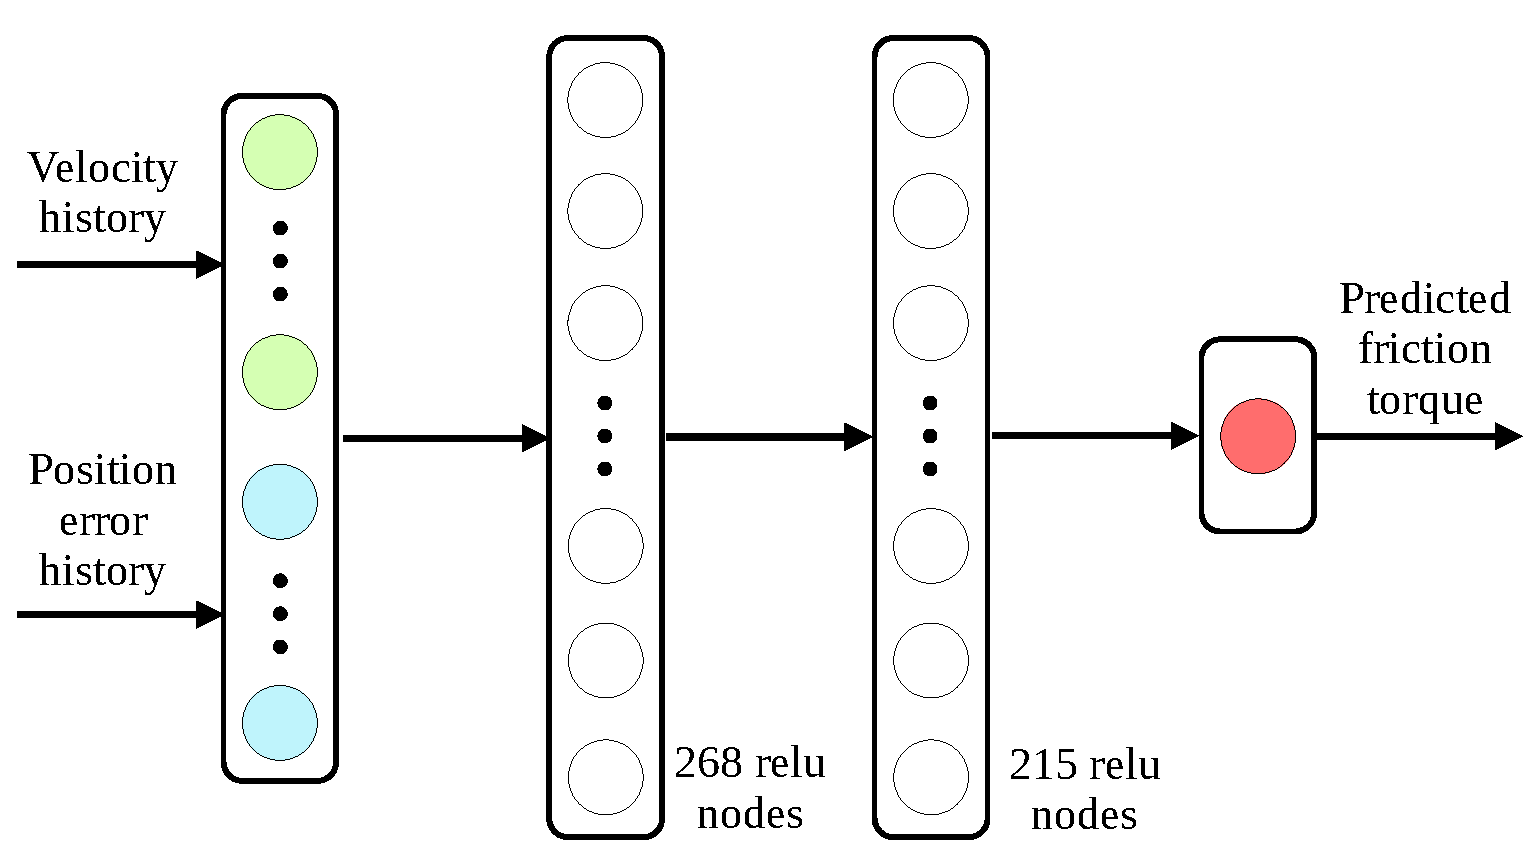
\includegraphics[width=0.85\linewidth]{figures/PINN.pdf}
    \caption{Neural Network architecture.}
    \label{fig:nnarchitecture}
    \vspace{-20pt}
\end{figure}

\subsubsection{Low-Level Torque Control}
The joint torques $\tau^{des}$ generated by the high-level controller described in Section \ref{sec:HLC}, are sent to the decentralized low-level joint torque controllers. The torque control schema is implemented as a feedforward controller including the compensation of the mechanical friction. The control law generates the reference currents to drive the motors.
\looseness=-1